% Settings for the default beamer theme
\documentclass[english, aspectratio=169]{beamer}
\usepackage[T1]{fontenc}
\usepackage[utf8]{inputenc}
\usepackage{tabularx}
\usepackage{babel}
\usepackage[ruled,vlined]{algorithm2e}
\SetAlgorithmName{Algoritmus}{algoritmus}{List of Algorithms}
\setcounter{secnumdepth}{3}
\setcounter{tocdepth}{3}

\makeatletter

\newcommand\makebeamertitle{\frame{\maketitle}}

% (ERT) argument for the TOC
\AtBeginDocument{%
  \let\origtableofcontents=\tableofcontents
  \def\tableofcontents{\@ifnextchar[{\origtableofcontents}{\gobbletableofcontents}}
  \def\gobbletableofcontents#1{\origtableofcontents}
}

% Theme settings
\usetheme{Frankfurt}
\usecolortheme{default}
\usefonttheme[onlymath]{serif}

% Template settings
\setbeamertemplate{navigation symbols}{}
\setbeamertemplate{blocks}[rounded][shadow=false]
\setbeamertemplate{title page}[default][colsep=-4bp, rounded=true, shadow=false]
\makeatother

\begin{document}

% Title page
\section{Bevezetés}
\title[]{Üzleti Intelligencia}
\subtitle{7. Előadás: Mesterséges mélytanulás}
\author[Kuknyó Dániel]{Kuknyó Dániel\\Budapesti Gazdasági Egyetem}
\date{2023/24\\1.félév}
\makebeamertitle

% Table of contents slide
\begin{frame}
\tableofcontents{}
\end{frame}

% Table of contents of the current section
\begin{frame}
\tableofcontents[currentsection]
\end{frame}

\begin{frame}{Biológiai és mesterséges neuronok}
\begin{columns}
\begin{column}{.5\textwidth}
Az ember találmányait mindig a természet ihlette. A repülőgépeket a madarak mintájára, a gépkocsit a lovak inspirálták. A természetes lépés ezután az volt, hogy az emberi agyat is modellezik.\par\medskip
Az első perceptron modellt Warren McCulloh és Walter Pitts hozta létre, először pedig Frank Rosenblatt épített egy perceptron gépet. Ez egy képfelismerő gép volt, 400 véletlenszerűen kapcsolt fotocella volt az érzékelője. A súlyokat potenciométerek implementálták, és a súlyok frissítését elektromotorok hajtották végre. 
\end{column}
\begin{column}{.5\textwidth}
\begin{center}
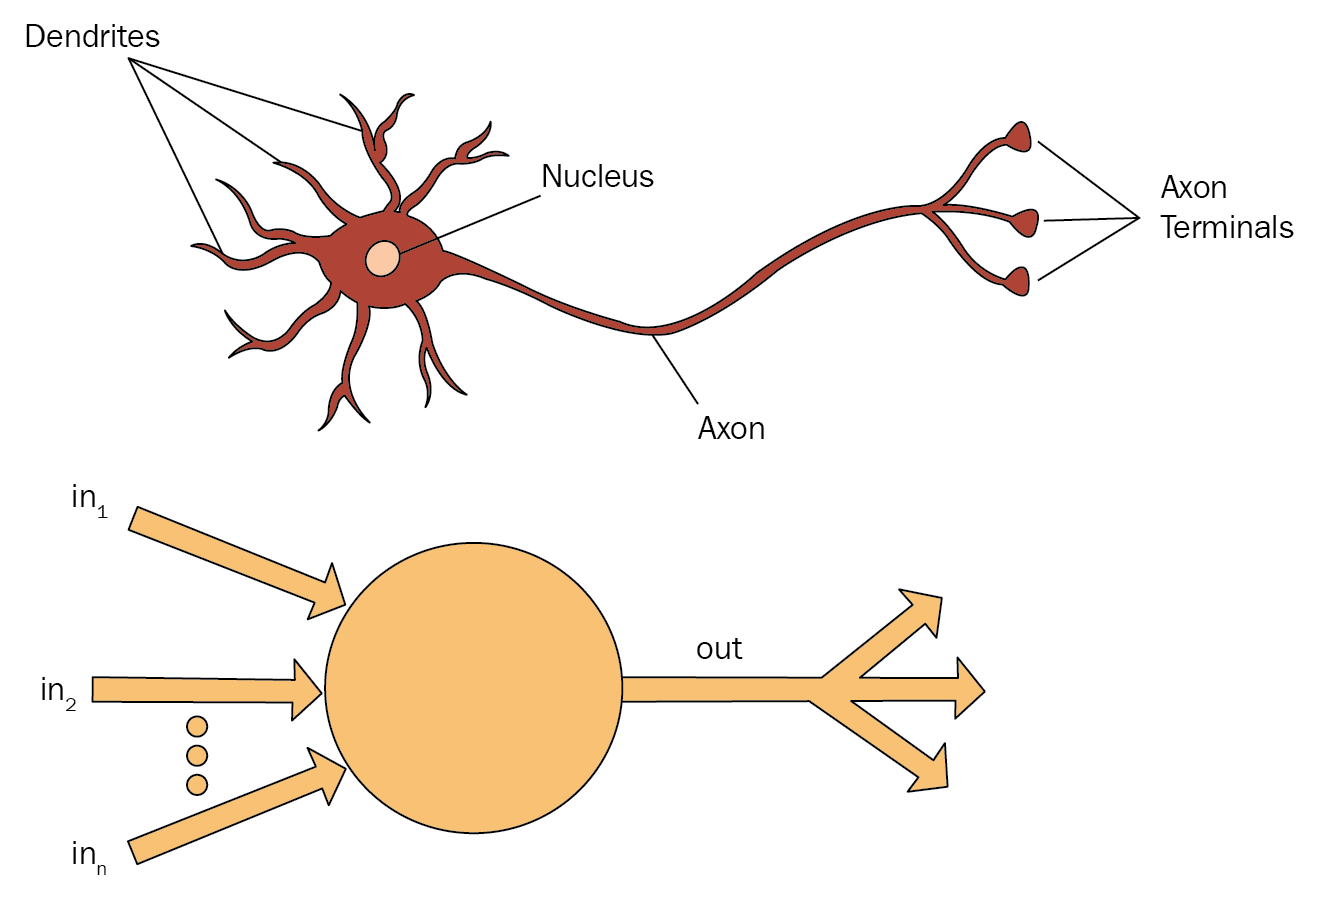
\includegraphics[width=7cm, keepaspectratio]{images/dl_1.png}
\end{center}
\end{column}
\end{columns}
\end{frame}

\begin{frame}{A neuron}
\begin{columns}
\begin{column}{.4\textwidth}
A neurális hálózatot \textbf{neuronok összessége} alkotja. Az egyes neuronok egyszerű elemi műveleteket végeznek. A neuronnak több inputja (kapcsolata) van, és mindegyikhez egy súly tartozik.\par\smallskip
A neuron kiszámítja az inputjainak a súlyozott összegét ($z=x_1w_1 + x_2w_2 + ... + x_nw_n$), majd ezt az értéket behelyettesíti egy aktivációs függvénybe ($o=\varphi(z)$). 
\end{column}
\begin{column}{.6\textwidth}
\begin{center}
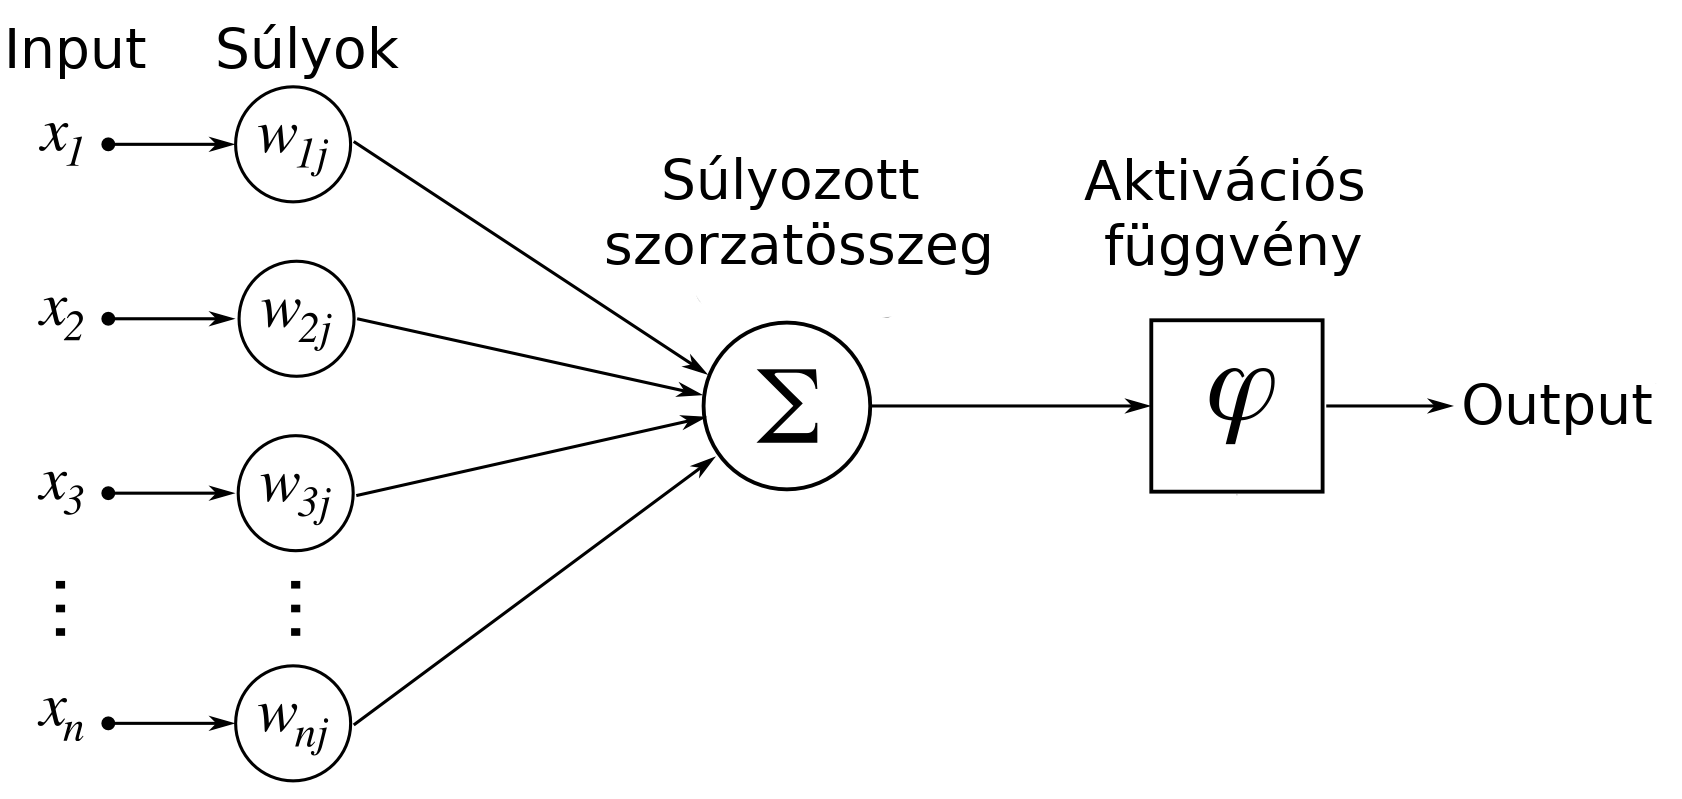
\includegraphics[width=9cm, keepaspectratio]{../../5_ql/doc/images/ql_21.png}
\end{center}
\end{column}
\end{columns}
\end{frame}

\begin{frame}{Gyakori aktivációs függvények}
\begin{columns}
\begin{column}{.5\textwidth}
A neuron által kiszámolt súlyozott szorzatösszeg egy aktivációs függvénybe kerül behelyettesítésre. \par\smallskip
A neurális hálózatok az aktivációs függvények segítségével \textbf{sajátítanak el komplex mintázatokat}. Az aktivációs függvény vezeti be a neurális hálózatokba a \textbf{nemlineáris transzformációt}, enélkül csak egy lineáris transzformáció lenne.\par\smallskip
A különböző alkalmazásokra külön aktivációs függvények használatosak.
\end{column}
\begin{column}{.5\textwidth}
\begin{center}
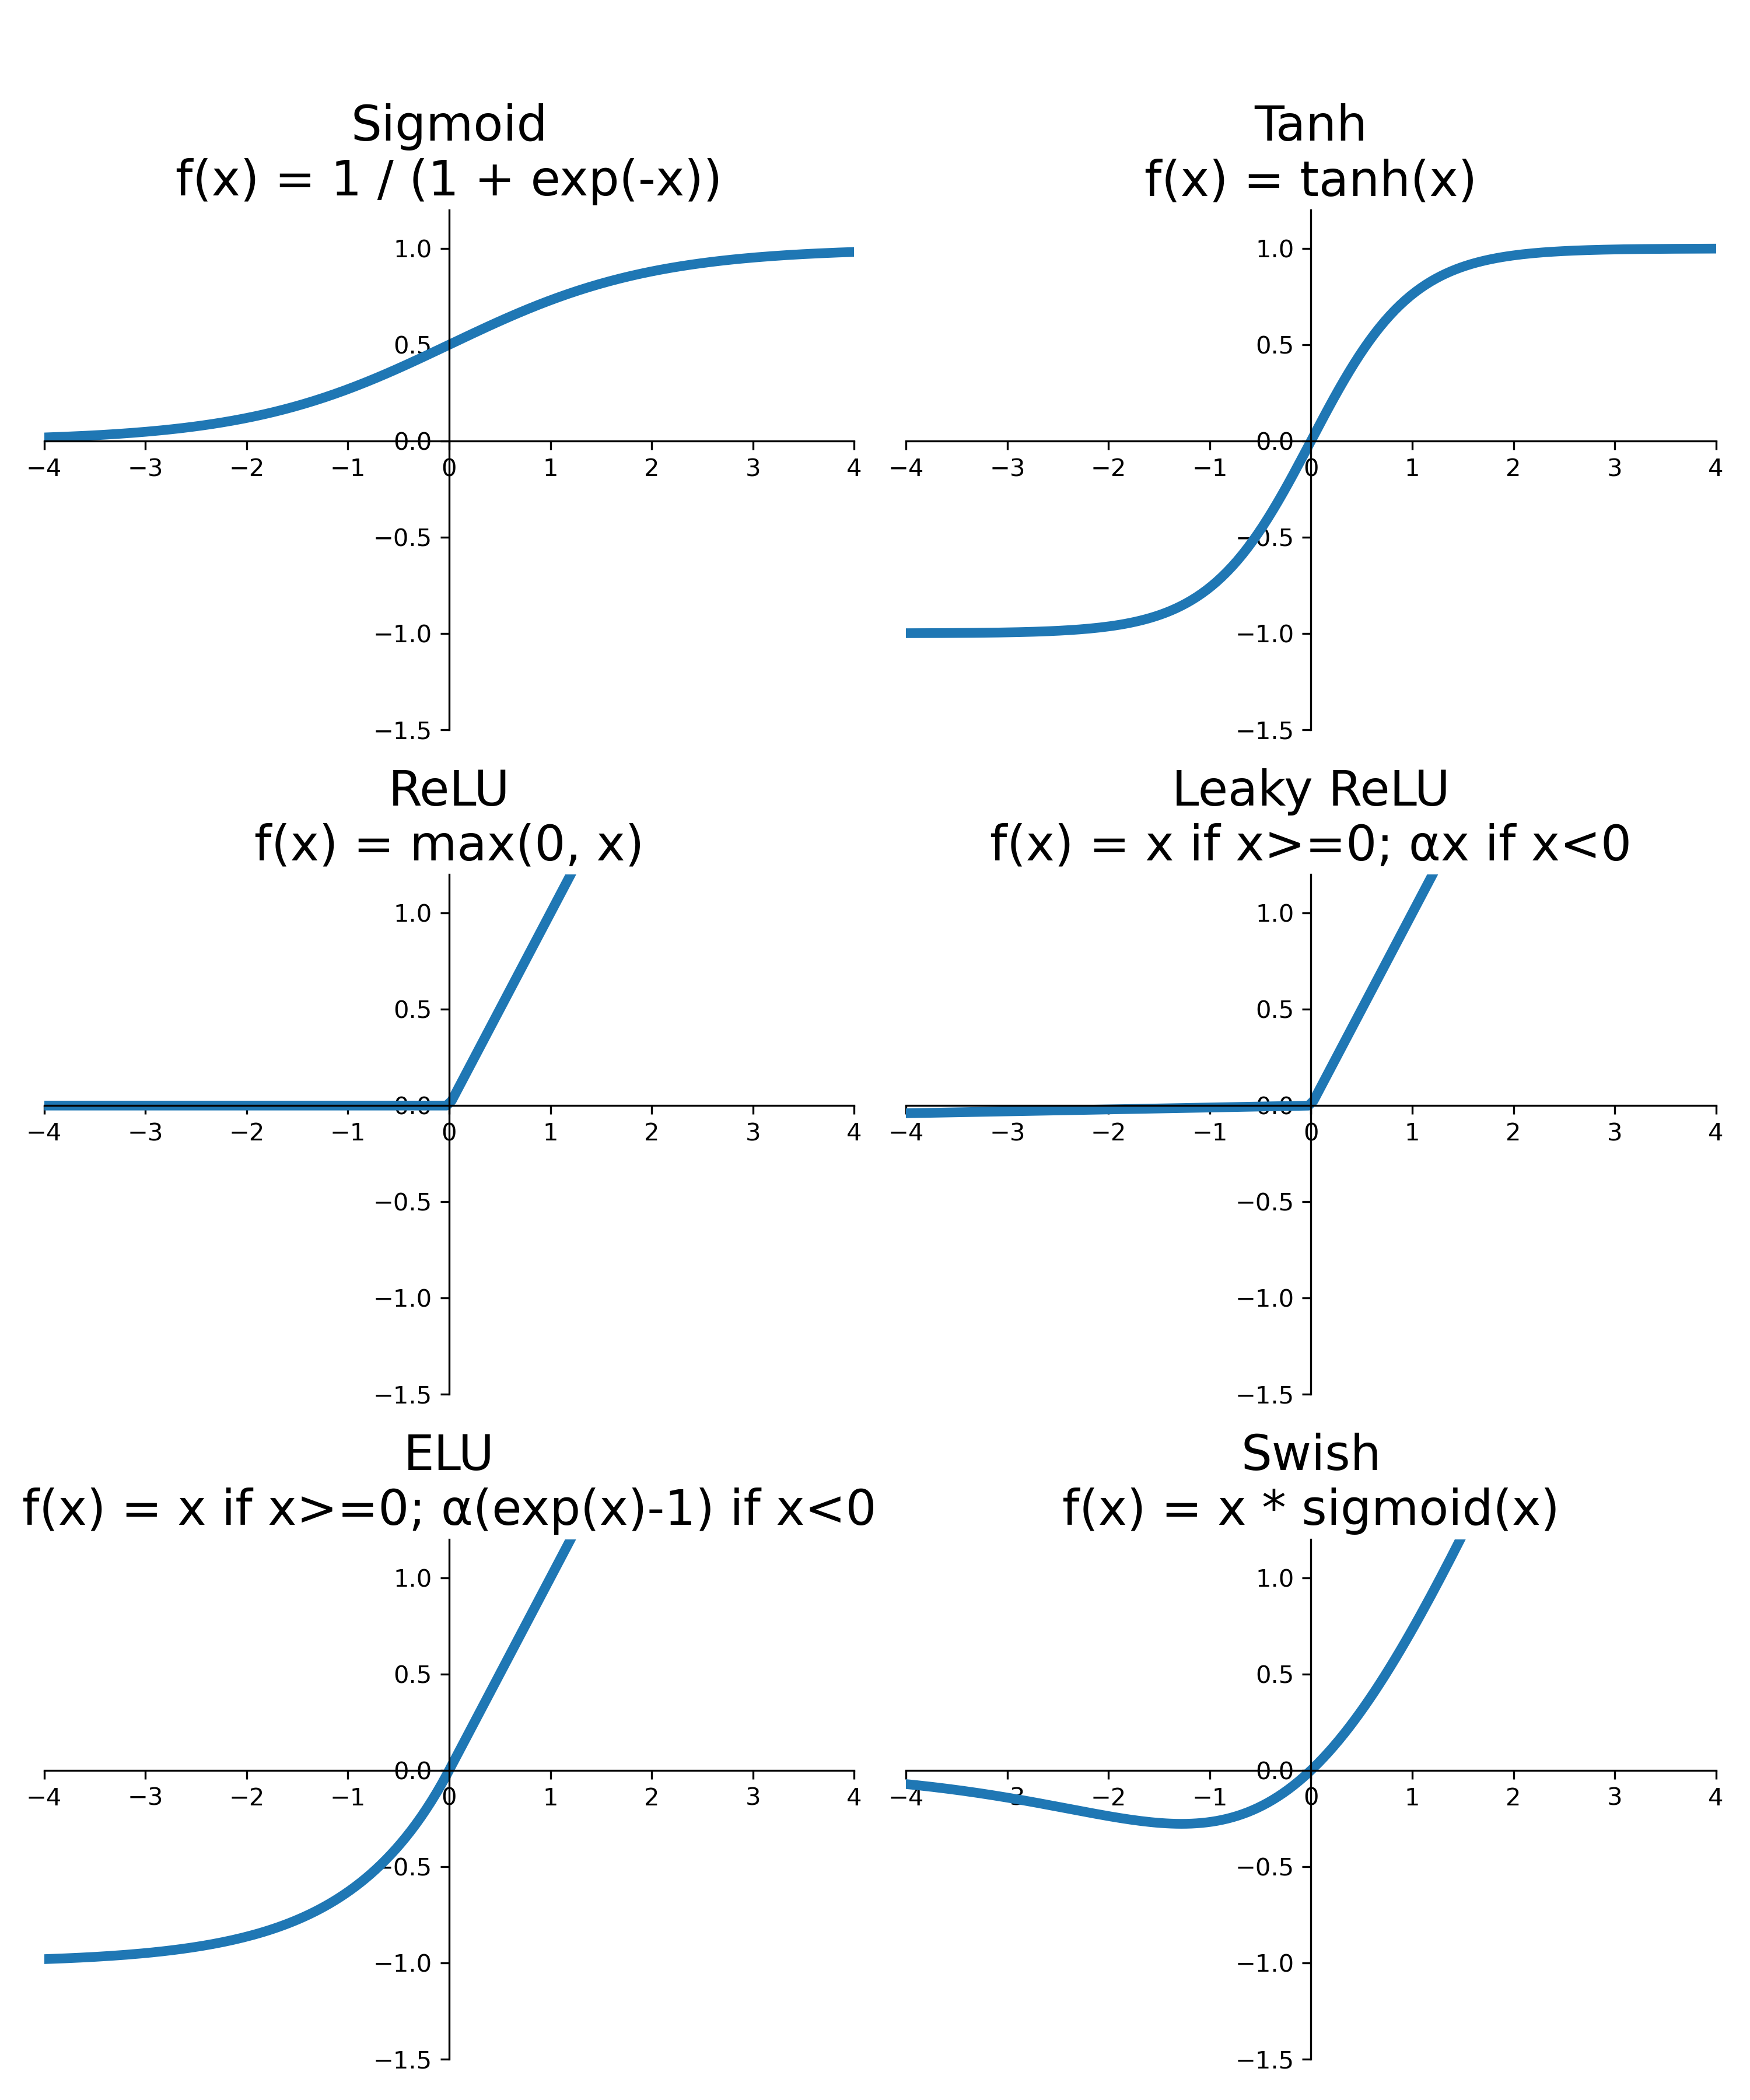
\includegraphics[height=7cm, keepaspectratio]{images/dl_2.png}
\end{center}
\end{column}
\end{columns}
\end{frame}

\begin{frame}{Többrétegű hálózatok}
\begin{columns}
\begin{column}{.5\textwidth}
Ebben az esetben a neuronok rétegekben foglalnak helyet. A kapcsolataik az előző réteg kimeneteivel állnak összeköttetésben. A legelső réteg neuronjai a bemeneti adattal állnak összeköttetésben. Minden bemeneti jellemzőhöz egy neuron tartozik.\par\smallskip
\begin{block}{Teljesen becsatolt neuronréteg kimenete}
\[
h_{w,b}(X)=\varphi(XW+b)
\]
\vspace{-0.5cm}
\begin{itemize}
	\item $X$: Input jellemzők mátrixa
	\item $W$: Kapcsolati súlyok mátrixa
	\item $b$: Torzítások vektora
	\item $\varphi$: Aktivációs függvény
\end{itemize}
\end{block}
\end{column}
\begin{column}{.5\textwidth}
\begin{center}
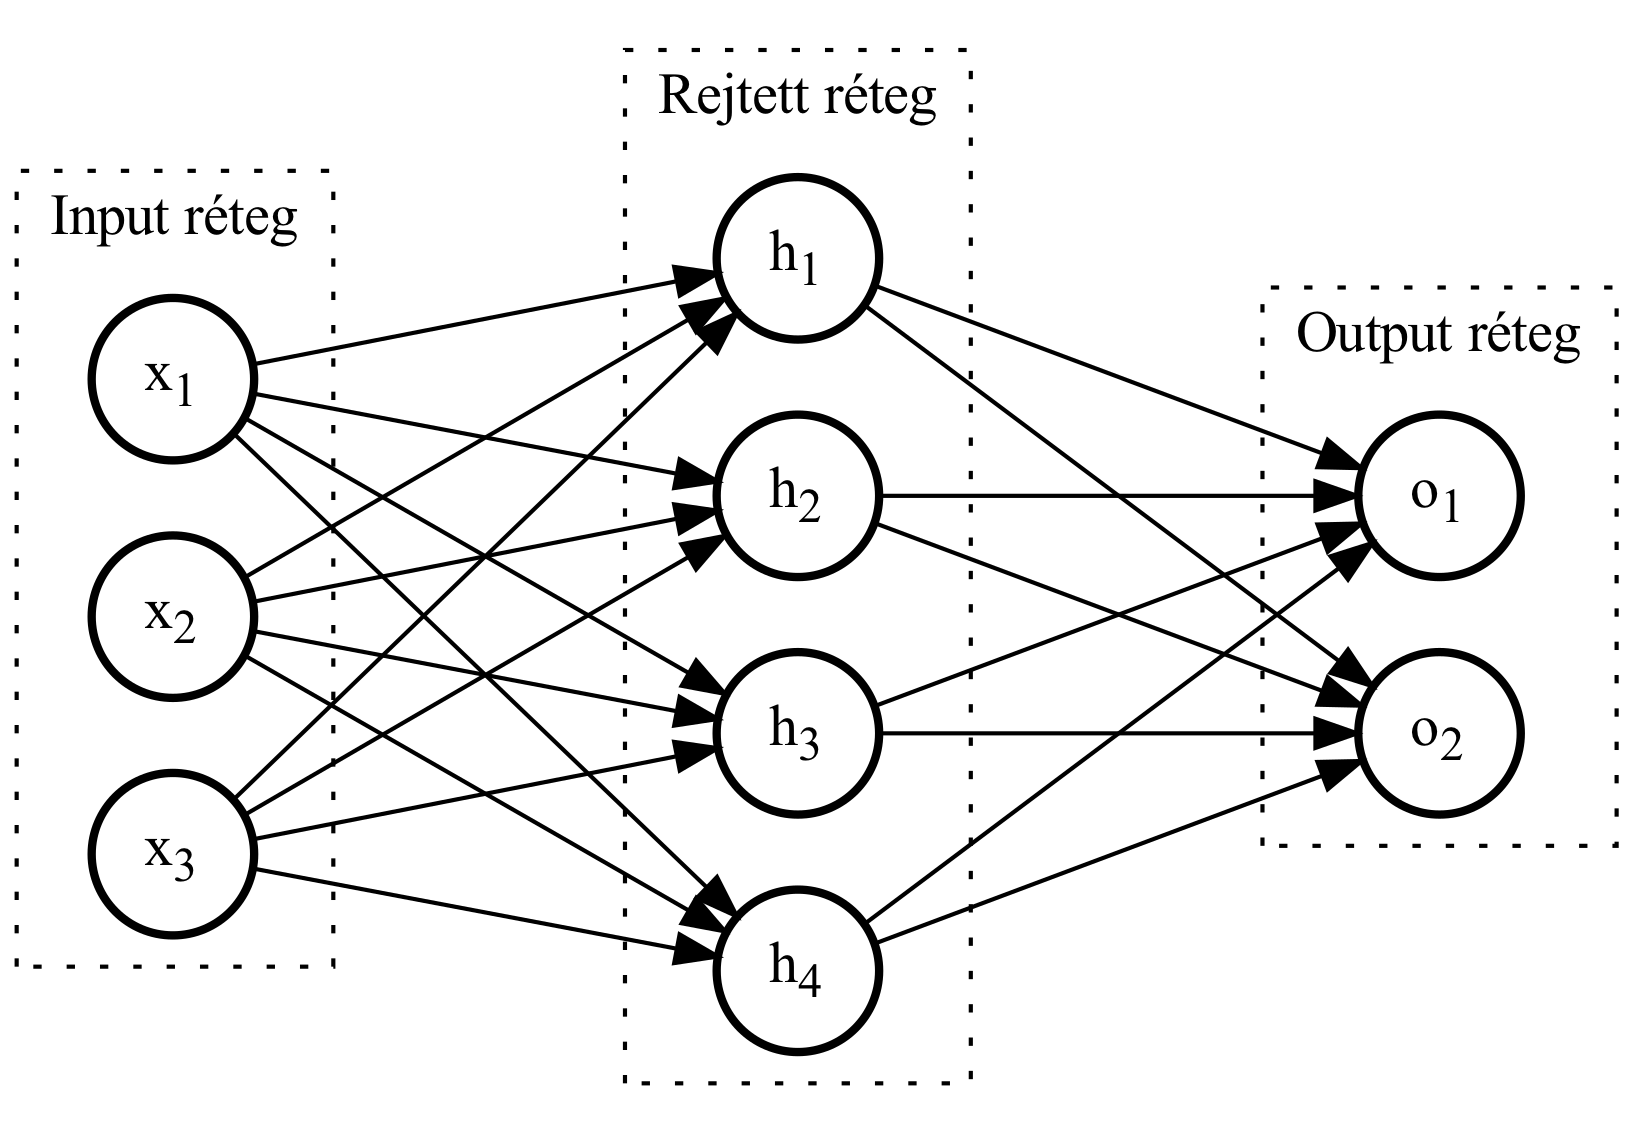
\includegraphics[width=7cm, keepaspectratio]{graphs/dl_0.png}
\end{center}
\end{column}
\end{columns}
\end{frame}

\begin{frame}{Hálózati architektúrák}
\begin{columns}
\begin{column}{.5\textwidth}
\only<1>{A regressziós problémák esetén a neurális hálónak \textbf{egyetlen output neuronja} van.\par\smallskip
A regresszió \textbf{tárgya egy folytonos} változó. Ebben az esetben a neuron output értéke a neurális hálózat predikciója a célváltozóra vonatkozóan.\par\smallskip
\textbf{Például}: hány fok lesz holnap este?\\
- 35.}
\only<2>{Az osztályozási problémák tárgya \textbf{egy diszkrét változó}, amely különálló kategóriákra osztható.\par\smallskip
Az osztályozó hálózatnak \textbf{annyi output neuronja van, ahány kategória lehetséges osztályozás esetén}. A predikció a mintaegyed adott osztályba esésének valószínűségét adja.\par\smallskip
\textbf{Például}: meleg vagy hideg lesz az idő holnap este?\\
- Hideg.}
\end{column}
\begin{column}{.5\textwidth}
\only<1>{\begin{center}
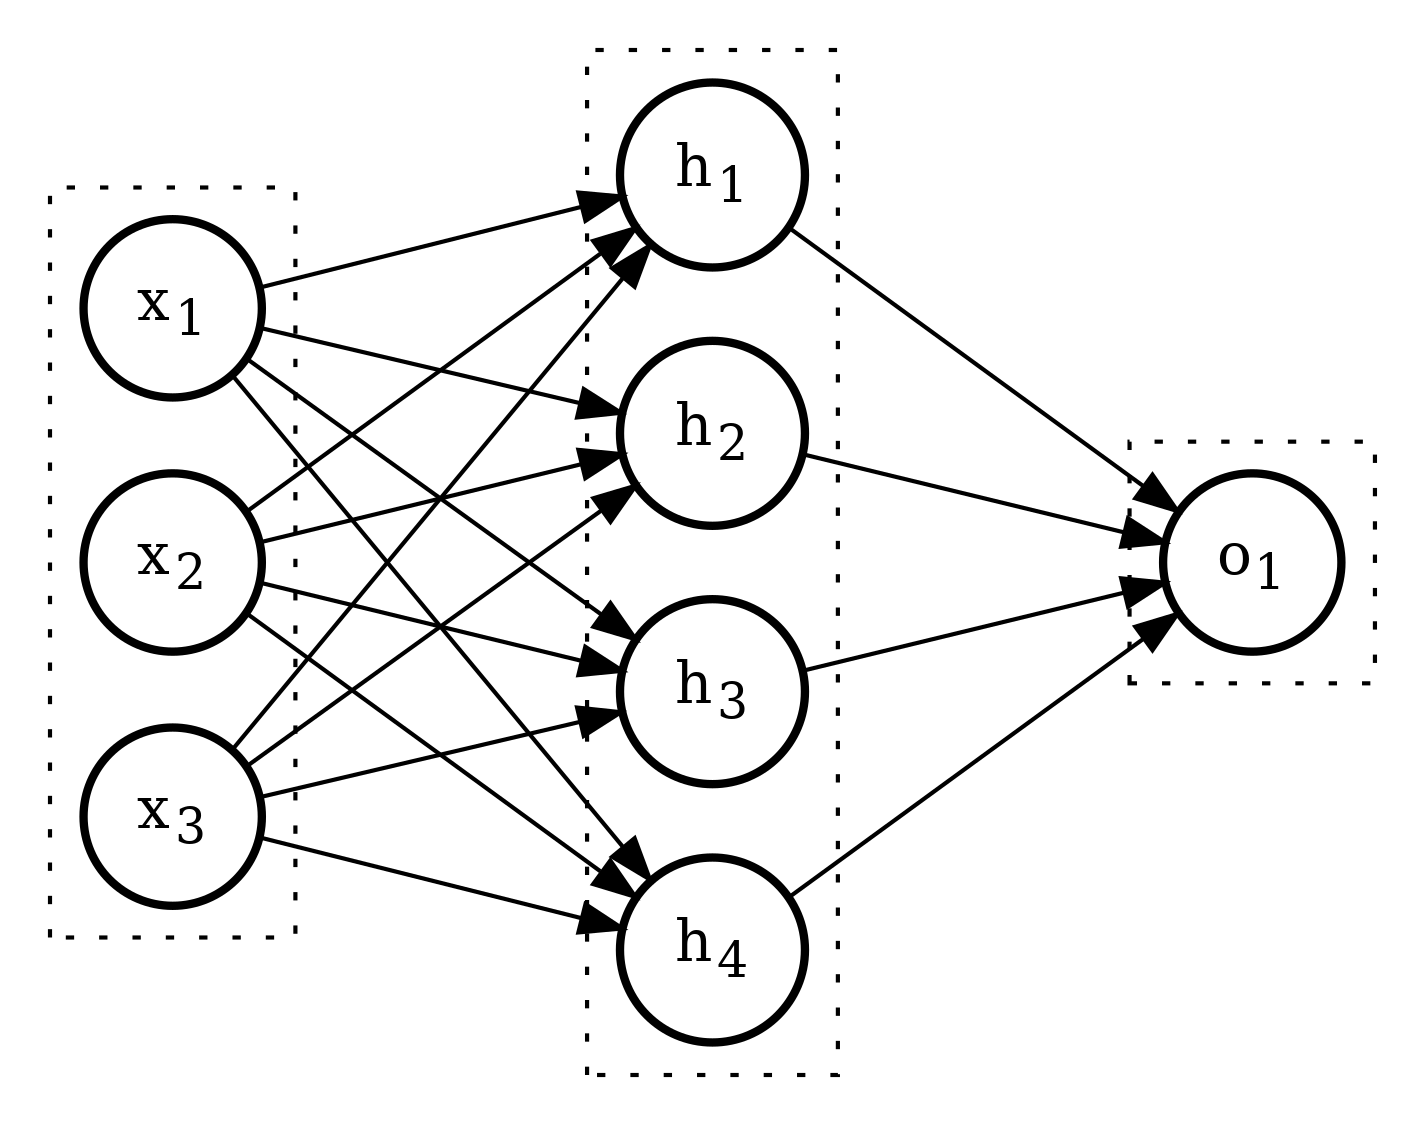
\includegraphics[width=7cm, keepaspectratio]{graphs/dl_2.png}
\end{center}}
\only<2>{\begin{center}
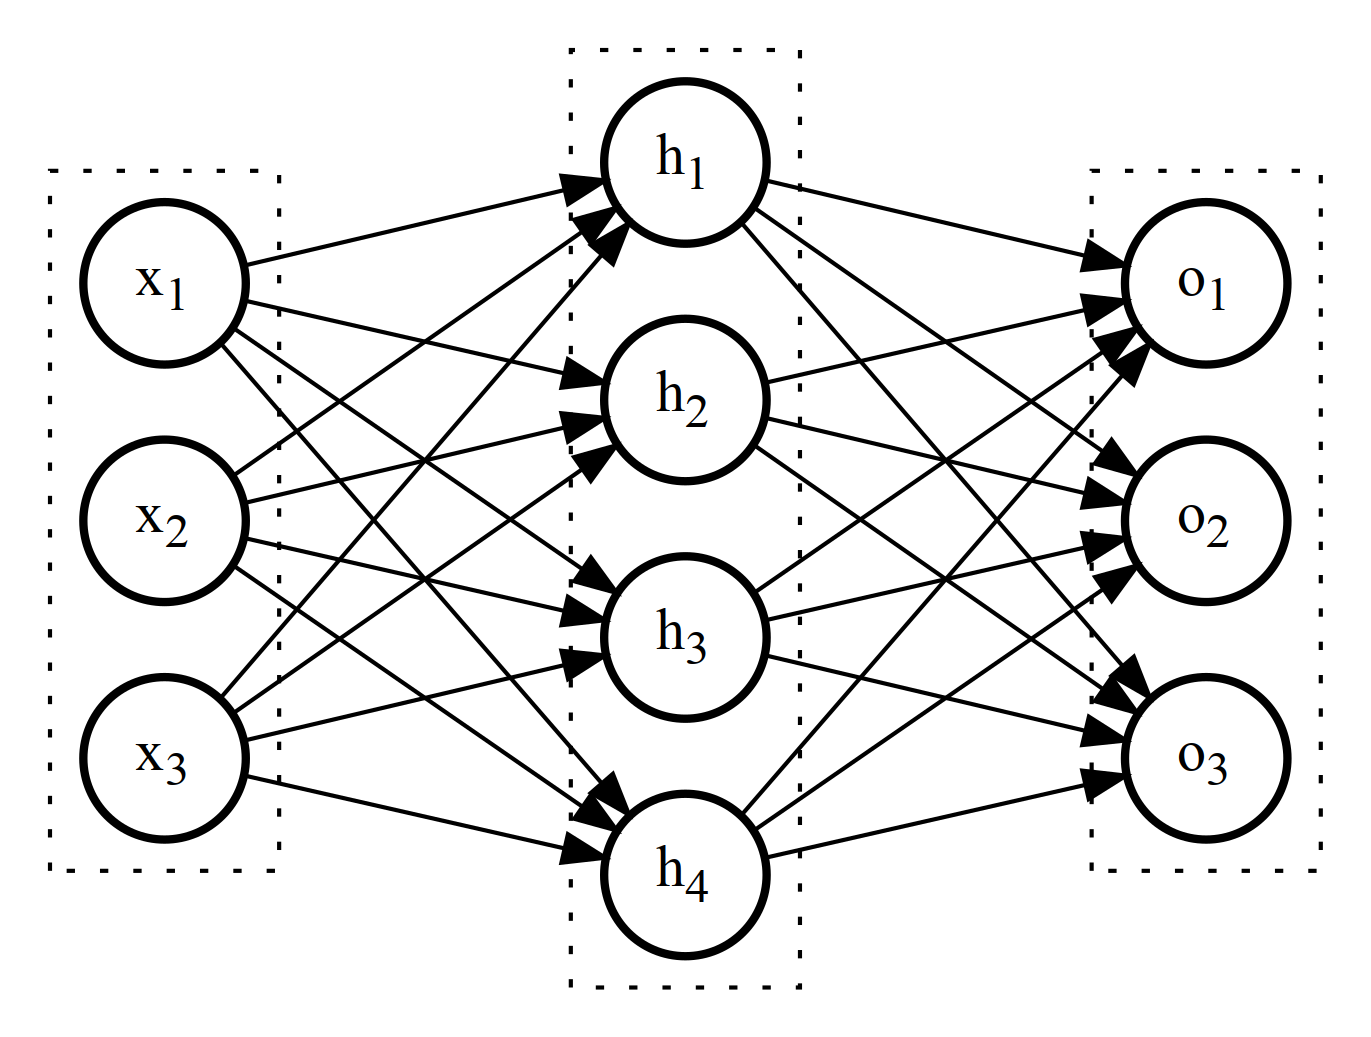
\includegraphics[width=7cm, keepaspectratio]{graphs/dl_1.png}
\end{center}}
\end{column}
\end{columns}
\end{frame}

\section{Neurális hálózatok tanítása}

\begin{frame}
\tableofcontents[currentsection]
\end{frame}

\begin{frame}{Hiba-visszaáramoltató algoritmus neurális hálózat súlyok tanítására}
\begin{enumerate}
	\item Inicializáció: a hálózat súlyainak és torzításainak kezdőértékeinek véletlenszerű megadása.
	\item Előreáramoltatás: minden tanító adatpontra a kötegben kiszámolja a rétegek output értékét: $h_{w,b}(X) = \varphi(XW + b)$.
	\item Költség kiszámítása: ez tetszőleges költségfüggvény esetén történhet. Regresszió esetében az átlagos eltérés-négyzet: $MSE = \frac{1}{n} \sum_{i=1}^n \left( y_i - f(x)_i \right)$
	\item 
\end{enumerate}
\end{frame}

\end{document}










